\documentclass{article}
\usepackage{indentfirst}
\usepackage[utf8]{inputenc}
\usepackage[margin=0.5in]{geometry}
\usepackage{graphicx}
\usepackage{verbatim}

\begin{document}

\title{Glossario di SWE}
\author{M9k}
\maketitle

%\section{TEXT}
%\subsection{TEXT}
%\subsubsection{TEXT}
%\paragraph{TEXT}
%\subparagraph{Subparagraph}Subparagraph text.\vspace{2mm}

\section{Introduzione}
	
	\subsection{Termini base}
		\textbf{Progetto}\\
		Insieme di attività e compiti\\
		-per raggiungere obbiettivi con specifiche fissate\\
		-data di inizio e di fine fissate\\
		-risorse limitate (es: persone, tempo, fondi, strumenti)\\
		-consuma risorse svolgendosi\\
			
		\textbf{Processo}\\
		\textit{Insieme di attività correlate} e \textit{coese} che trasformano ingressi (bisogni) in uscite (prodotti) secondo regole date, consumando risorse nel farlo\\
		Correlate: hanno un motivo/una capacità per stare assieme\\
		Coese: utili al medesimo obiettivo\\
		
		\textbf{Attività}\\
		Cosa da fare, che voglio fare, per il raggiungimento degli obbiettivi, composta da più compiti\\
		
		\textbf{Compito}\\
		Cosa che una persona deve fare, che va fatta\\

		\textbf{Fasi principali:}\\
		-Pianificazione (\textit{gestione risorse} e \textit{responsabilità})\\
		-Analisi dei requisiti (\textsl{cosa} devo fare)\\
		-Progettazione (\textit{come} farlo)\\
		-Realizzazione (con una \textit{qualità}, \textit{verificando} la correttezza, \textit{validando} i risultati)\\
		
		\textbf{Efficienza}\\
		Produttività, metrica del grado di riduzione degli sprechi\\
		Quantità prodotto realizzato/risorse utilizzate\\
		
		\textbf{Efficacia}\\
		Qualità, metrica del grado di raggiungimento degli obbiettivi interni (del fornitore) o esterni (gradimento del cliente)\\
		
		\textbf{Iterazione}\\
		Può essere anche un incremento, procedere per raffinamento o rivisitazioni (pittura)\\
		Non so se sto migliorando o meno, non quantificabile, non efficiente, rifinisco gli aspetti senza magari avanzare, non so a che punto sono\\
		
		\textbf{Incremento}\\
		Procedere per aggiunta a un impianto base (scultura)\\
		Si progredisce a punti, a baseline, quantificabile\\
		
		\textbf{Prototipo}\\
		Per provare e capire meglio, usa e getta (bozza), oppure per avere avanzamento incrementale (baseline)\\
		
		\textbf{Baseline}\\
		Prototipo da utilizzare come base, come punto d'appoggio per le successive attività\\
		
		\textbf{Prodotto SW}\\
		È un insieme di parti, che stanno assieme secondo la loro \textit{configurazione}.\\
		Ogni sistema fatto di parti va gestito con il \textit{controllo di configurazione}.\\
			
		\textbf{Configurazione}\\
		Modo nel quale si assemblano i pezzi di un software (ordine, parti, librerie, impostazioni, etc)\\
		Usato per il build, si gestisce con il controllo di configurazione\\
			
		\textbf{Metrica}\\
		Metodo di misurazione, l'unità di misura da sola è insignificante\\
		
		
		
		
		
		
		
		
		
		
		
		
		
		
		
		
		
		
			
	\clearpage
	\subsection{Ingegneria}
		\textbf{Ingegneria}\\
			Applicazioni principi matematici e scientifici a scopo pratico, NON per esplorare nuove possibilità o espandere la scienza\\
			Mai inventare, utilizzare sempre metodi testati e funzionanti\\
			
		\textbf{Best practice}\\
		Miglior modo (way of working) per raggiungere uno scopo, secondo applicazioni passate che hanno dimostrato i risultati\\
		
		\textbf{Pratical ends}\\
		Avere un fine civile e sociale oltre che economico\\
		
	\subsection{Ingegneria del software}
		\textbf{Ingegneria del software}\\
		Disciplina per la realizzazione di \textit{prodotti software} impegnativo e che richiede collaborazione\\
		-in grande e in piccolo (tanto in quantità o poco e specializzato)\\
		-con qualità = \textit{efficacia} = grado di conformità, capacità di raggiungere gli obiettivi\\
		-con costi e tempi contenuti = \textit{efficienza} = capacità di ridurre le risorse e gli sprechi, seguendo la best practice \\
		-tutto lungo il \textit{ciclo di vita}\\
		
		\textbf{Ingegneria del software}\\
		Raccogliere, organizzare e consolidare conoscenza (body of knowledge) necessarie a realizzare progetti SW con massima efficacia e efficenza.\\
		Acquisire, utilizzare e mantenere i best practice.\\
		
		
		\textbf{Ingegneria del software}\\
		Secondo IEEE: Approccio \textit{sistematico}, \textit{disciplinato} e \textit{quantificato} allo sviluppo, uso, manutenzione e ritiro del SW.\\
		Sistematico: metodico e rigoroso, usando una metodologia precisa, per studiare ed evolvere best practice\\
		Disciplinato: regole fissate\\
		Quantificabile: efficienza ed efficacia misurabili.\\
		
		
		\textbf{Tipologie di prodotti software}\\
		-Commessa: forma, contenuto e funzioni definiti dal committente\\
		-Pacchetto: forma, contenuto e funzioni idonei alla replicazione\\
		-Componente: forma, contenuto e funzioni idonei alla composizione\\
		-Servizio: forma, contenuto e funzioni definiti dal problema\\
		
		\textbf{Le 4 P di SWE}\\
		-People (stakeholder e team di sviluppo)\\
		-Product (SW e documentazione)\\
		-Project (Insieme di attività di produzione)\\
		-Process (way of working)\\
		
		\textbf{Ciclo di vita}\\
		Insieme di stati di avanzamento del software fino al ritiro\\
		Un ciclo di vita lungo porta a elevati costi di \textit{manutenzione}\\
		
		\textbf{Manutenzione}\\
		-correttiva: fix dei bug\\
		-adattiva: rifinisco i requisiti\\
		-evolutiva: evoluzione del software secondo i nuovi usi\\
		
		\textbf{Utilità}\\
		\textit{Metrica} riguardante gli utilizzi/utenti di un prodotto nel tempo\\
		
		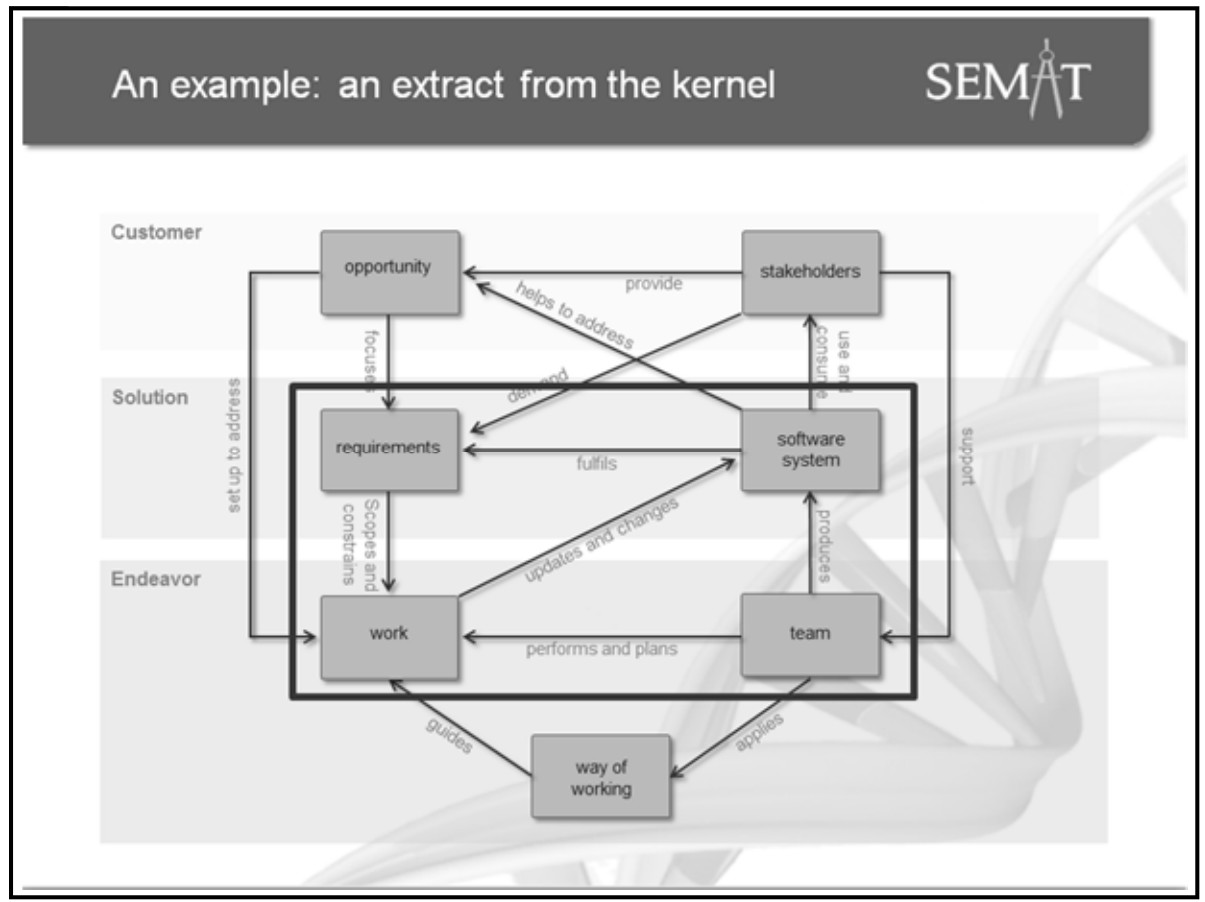
\includegraphics[width=14cm]{semat_org.jpg}\\
		
		
	\clearpage
	\section{Processi SW}
		\textbf{Ciclo di vita}\\
		Gli stati che il prodotto assume dal concepimento al ritiro\\
		Serve per valutare costi, tempi, obblighi e rischi PRIMA di svolgere il progetto\\
		Scelta tra più possibili cicli di vita, ognuno con vantaggi e limiti\\
		
		\textbf{Processi di ciclo di vita}\\
		Specificano le attività da svolgere per abilitare corrette transizioni di stato nel ciclo di vita\\
		
		
		\textbf{Modelli di ciclo di vita}\\
		Descrivono come i processi di ciclo di vita si relazionano tra di loro rispetto agli stati\\
		Aiutano a pianificare, organizzare ed eseguire lo svolgimento delle attività\\
		Svariati, scelgo in base alla situazione, ognuno con pregi e limiti\\
		
		\textbf{Ciclo di sviluppo}\\
		Ciclo di vita fino alla consegna, senza utilizzo, manutenzione e ritiro\\
		
		\textbf{Visione a grafi}\\
		Gli stati sono i nodi (concezione, sviluppo, utilizzo, ritiro, etc), gli archi le attività svolte sul prodotto necessarie per farlo avanzare.\\
		Natura degli stati e pre- e post- condizione determinate da \textit{obblighi} (vincoli contrattuali), \textit{regole} (standard di processo) e \textit{strategie}\\
		
		\textbf{Modelli più significativi}\\
		-Sequenziale o a cascata (waterfall)\\
		-Incrementale\\
		-A evoluzioni successive\\
		-A spirale\\
		-Per componenti\\
		-Agile\\
		
		\textbf{Riuso}\\
		-Occasionale: copia-incolla, basso costo, scarso impatto, da evitare\\
		-Sistematico: per progetto/prodotto/azienda, maggior costo, maggior impatto\\
		
		\textbf{Malleabilità}\\
		Un buon software non è statico, ma si modifica e si addatta in quanto usandolo si scoprono migliorie e/o cambiano gli usi\\
			
		\textbf{Processo}\\
		\textit{Insieme di attività correlate} e \textit{coese} che trasformano ingressi (bisogni) in uscite (prodotti) secondo regole date, consumando risorse nel farlo\\
		Correlate: sono collegate, hanno la capacità di stare assieme\\
		Coese: hanno un motivo di stare assieme\\
		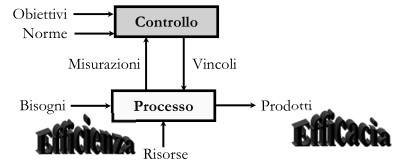
\includegraphics[width=14cm]{processi.jpg}\\
		Risorse: efficienza = produttività, cosa ho fatto/quante risorse ho utilizzato\\
		Misurazione: efficacia, raggiungimento di obbiettivi interni (del fornitore, cioè di chi crea il software) o esterni (gradimento da parte del cliente)\\
		
		\textbf{Economicità}\\
		Insieme di efficienza ed efficacia, da controllare DURANTE lo sviluppo usando:\\
		-dati tempestivi (non si può attendere la fine, sarebbe troppo tardi)\\
		-dati accurati (niente opinioni personali ma numeri)\\
		-non intrusività (non bloccare il lavoro per controllare il progresso)\\

		\textbf{Standard di processo}\\
		Voluti dai committenti per vincolare il fornitore\\
		Per facilitare \textit{controllo}, \textit{collaudo} e \textit{accettazione}\\
		Settoriali o generali/trasversali\\
		Vincolo (imposto) o riferimento (non imposto, come modello)\\
		
		\textbf{Standard come modello di azione}\\
		Sono una serie di passaggi da compiere, guida passo a passo, come una ricetta\\
		Definizione e imposizione di \textit{procedure}, definizione e proposizione di \textit{processi da specializzare}\\
		
		\textbf{Standard come modello di valutazione}\\
		Servono per avere una valutazione sul comportamento del progetto\\
		Modelli più generali, copre più contesti, per identificare best practice\\
	
		\textbf{ISO/IEC 12207:1995}\\
		Letta come 12 207\\
		Più diffuso, ad alto livello, molto astratto, preso spunto dagli standard militari del dipartimento di difesa\\
		Identifica i processi di ciclo di vita del SW\\
		Struttura modulare che richiede specializzazione\\
		Specifica le responsabilità sui processi e i prodotti\\
		Tre parti principali: processi primari, di supporto e organizzativi\\
	
		\textbf{Processi primari}\\
		Necessari per l'esistenza di un progetto\\
		ES:\\
		-Fornitura (gestione rapporti con il cliente, primo passo di un progetto)\\
		-Acquisizione (gestione dei sotto-fornitori)\\
		-Sviluppo\\
		-Gestione operativa (utilizzo, erogazione, installazione)\\
		-Manutenzione (correzione, adattamento, evoluzione)\\
		
		\textbf{Processi di supporto}\\
		ES:\\
		-Documentazione\\
		-Accertamento qualità\\
		-Gestione delle versioni e delle configurazioni\\
		-Qualifica: verifica + validazione\\
		-Revisioni congiunte con il cliente\\
		-Verifiche ispettive interne\\
		-Risoluzione dei problemi (gestione dei cambiamenti)\\
		
		\textbf{Processi organizzativi}\\
		ES:\\
		-Gestione dei processi\\
		-Gestione delle infrastrutture\\
		-Miglioramento del processo\\
		-Formazione personale\\
		
		\textbf{Tecniche}\\
		Ricette per svolgere determinati compiti\\
		Vincoli o strategie restringono il grado di libertà\\
		
		\textbf{Buona organizzazione}\\
		Si basa sul riconoscere i processi, adottarli consapevolmente ed efficacemente e supportarli in modo efficiente\\
		
		\begin{comment}
			\textbf{Tipi di processo}\\
			-Standard: di base, generico, condiviso tra aziende nello stesso dominio applicativo\\
			-Definito: specializzazione per adeguare un processo standard a caratteristiche aziendali\\
			-Di progetto: istanziato, usano risorse aziendali per raggiungere obbiettivi prefissati e con tempo limitato (progetti)\\
			
			\textbf{Processi specializzati/definiti}\\
			-Chiari, stabili, documentati\\
			-indipendenti dal modello di ciclo di vita adottato\\
			-Indipendenti dalle tecnologie\\
			-Indipendenti dal dominio applicativo\\
			-Indipendenti dalla documentazione richiesta\\
			
			\textbf{Processi di progetto}\\
			-Ben pianificati\\
			-Chiare scelte di specializzazione (definire lo scenario, le attività e i compiti aggiuntivi e specifici, organizzare le relazione tra i processi specializzati)\\
			-Massima attenzione nel condurre il progetto\\
			-Valutazione critica dell'esito (formalizzare le parti che operano bene)\\
			
			\textbf{Dipendono da:}\\
			-Dimensione del progetto\\
			-Complessità del progetto\\
			-Rischi identificati (da dominio applicativo e tecnologie)\\
			-Competenze ed esperienza delle risorse umane\\
			-Fattori dipendenti dal contratto\\
		\end{comment}
		
		\textbf{Organizzazione interna}\\
		Principio del miglioramento continuo:\\
		-Plan: definire attività, scadenze, responsabilità, risorse per raggiungere obbiettivi di miglioramento\\
		-Do: eseguire secondo i piani\\
		-Check: verificare l'esito delle azioni di miglioramento rispetto le attese\\
		-Act: applicare soluzioni correttive alle carenze\\
		
		\textbf{Processi e modelli di ciclo di vita}\\
		-La specifica dei processi non determina il modello di ciclo di vita\\
		-Il livello di coinvolgimento del cliente determina natura, funzione e sequenza dei processi di revisione\\
		-Quando il SW è parte di un sistema complesso il modello di ciclo di vita a \textit{livello di sistema} è spesso sequenziale.\\
		
		\textbf{Influenze sul modello di ciclo di vita}\\
		-Politiche di acquisizione e di sviluppo (versione unica o multipla, dipendenza da/verso altre componenti)\\
		-Natura, funzione e sequenza dei processi di revisione (interne, esterne, non bloccanti)\\
		-Necessità/utilità di fornire evidenze preliminari di fattibilità (prototipi bozza o baseline, studi e analisi preliminari)\\
		-Esigenza di iterazioni o di configurazioni (build, deployment)\\
			
			
			
			
	\clearpage
	\section{Ciclo di vita}
	
		\textbf{Stati principali}\\
		-Concezione\\
		-Sviluppo\\
		-Utilizzo\\
		-Ritiro\\
		
		\textbf{Organizzare le attività di processo}\\
		Si devono identificare dipendenze tra ingressi ed uscite, poi fissarle nel tempo assieme ai criteri di attivazione (pre-condizioni) e di completamento (post-condizioni)\\
		
		\textbf{Fase}\\
		Stazionamento in uno stato del ciclo di vita o in una transizione tra stati\\
		
		\textbf{Sistema di qualità}\\
		Associato al modello per assicurare conformità e maturità\\
		
		
		\textbf{Modello a cascata o sequenziale}\\
		Fasi:\\
		-Analisi (requisiti di sistema e software, etc)\\
		-Progettazione (Design, etc)\\
		-Realizzazione (Codifica, integrazione, collaudo, etc)\\
		-Manutenzione\\
		Eseguite in modo rigidamente sequenziale, no parallelismo, guidato da documentazione, codice solo alla fine, con pre-condizioni e post-condizioni per ogni fase\\
		Eccessiva rigidità, non permette modifiche ai requisiti, necessita di molta manutenzione, molto burocratico e poco realistico\\
		Big-gan integration: si integra tutto alla fine in un solo colpo, se non funziona difficile isolare e correggere il problema\\
		\textbf{Correzioni}\\
		-Prototipazione: usa e getta, scrivendo la documentazione si fanno delle prove\\
		-Cascata con ritorni: torno indietro per correggere/rifare una parte, rompendo il modello, iterazioni! - Modello iterativo\\
		
		\textbf{Modello iterativo}\\
		Applicabile a qualsiasi altro modello, consente l'adattamento (a evoluzione dei problemi, requisiti, soluzioni e tecnologie)\\
		Si ritorna indietro rispetto l'asse temporale\\
		
		\textbf{Modello incrementale}\\
		Fasi:\\
		-Define outline requiments\\
		-Assign requiments to increments (essenziale per poter procedere a incrementi)\\
		-Design system architecture (come le parti si compongono, essenziale per il parallelismo)\\
		finchè non ho il sistema finale:\\
		|-Develop system increment\\
		|-Validate increment\\
		|-Integrate increment\\
		|-Validate system\\
		Possibile svolgere gli incrementi in parallelo\\
		Riassumibile in : ``Analisi e progettazione'', poi ciclo su ``Progettazione di dettaglio'' e ``Implementazione dettaglio''\\
		
		\textbf{Modello evolutivo}\\
		Per uno scenario che varia (es Browser), molteplici versioni intermedie, ogni fase ammette iterazioni multiple e parallele\\
		
		\textbf{Modello a componenti}\\
		Si basa sul riutilizzo di componenti\\
		Fasi:\\
		-Analisi requisiti\\
		-Analisi componenti\\
		-Adattamento bisogni ai requisiti (controllo cosa fa al caso mio e come dovrò modificarlo per soddisfare i requisiti)\\
		-Progettazione con riuso\\
		-Sviluppo e integrazione\\
		-Validazione di sistema\\
		
		\textbf{Modelli agili}\\
		-Niente regole rigide\\
		-Il software funzionante è più importante di una buona documentazione\\
		-Collaborare con il cliente, non negoziare\\
		-Essere reattivi, non mirare alla pianificazione\\
		Ma:\\
		-Adattare le regole è ok, ma bisogna mantenere un occhio su costi/benefici\\
		-La mancanza della documentazione fa lievitare il costo di manutenzione\\
		-Non pianificare significa non sapere se si sta avanzando e i rischi che si corrono\\
		\textbf{User story}\\
		Minuta, resoconto con il cliente, dialogando specifica i problemi e i requisiti, pezzo per pezzo\\
		Sarà una lista di cose che vuole, che preferirebbe e che non vuole, da usare per controllare l'avanzamento e l'efficacia\\
		\textbf{3 forme principali}\\
		La maggiore: \textbf{SCRUMB}\\
		Iterazione controllata, c'è un \textit{backlog} di cose da svolgere, si sceglie quali fare (\textit{sprint}) prendendo le più utili/necessarie/importanti, le faccio, le unisco in un incremento e itero nuovamente\\
		Sprint usualmente di circa 2 settimane, con misurazioni giornaliere brevi di tipo stand-up, intrusive!\\
		
		\textbf{Il ciclo di vita secondo SEMAT}\\
		Utilizzo di checklist comuni per controllare l'avanzamento e l'aver completato le principali problematiche dei vari ambiti (opportunità, stakeholder, requisiti, sistema software, team, lavoro e way-of-working)\\
		
		
	\clearpage
	\section{Nuovo argomento}
	
\end{document}
